\begin{figure}
\centering
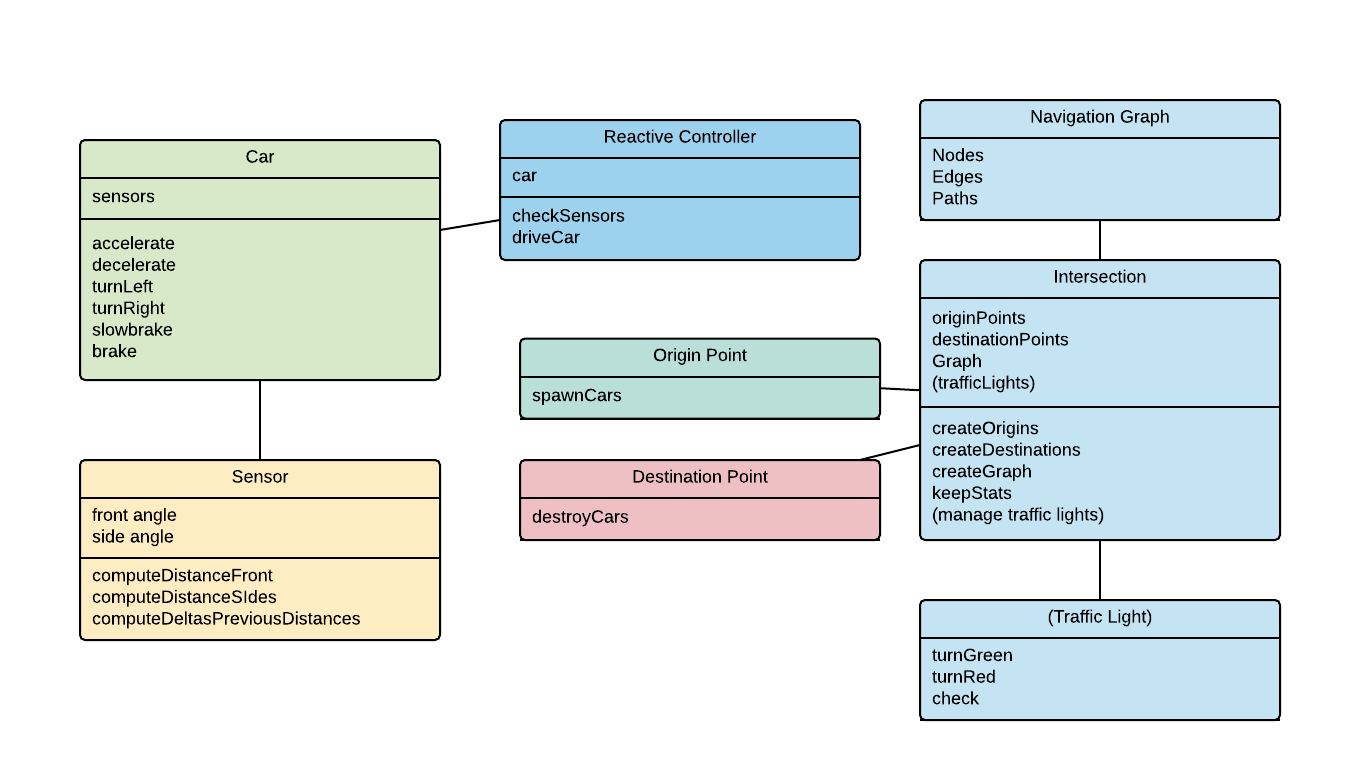
\includegraphics[scale=.6]{img/classdiagram}
\caption{Overview of Unity3D software package}
\label{figure:classdiagram}
\end{figure}

As we have settled on using Unity3D we work within its boundaries.
It is component driven, meaning every object in the world consists of a collection of components and a transform - the transform is the objects spatial information.
These components can be either colliders, renderers, or custom scripts, and objects can contain other objects - they can be composite.

The implementation was done by splitting the work in three major blocks. One was \textit{the vehicle model}, another was \textit{the intersection model} and the last \textit{the reactive controller} for the car.
An overview of our software package is depicted on figure \ref{figure:classdiagram}.

\begin{itemize}
%\item Presentation of our model.
%\item Intersection w/wo traffic lights. Cars going straight vs. cars turning.
%\item Car model and sensor modelling (sick vs simplified directional).
%\item Graph for navigation.
%\item Reactive controller.
%\item Special rules (right hand).
\item Sensor range limitation based on braking distance considerations.
\item SimScale to RealWorldScale
\end{itemize}

\subsection{The World Model}
As observed in the real world, multiple intersection models exist, three lane and 4 lane intersections are the most common ones.
The style can be either with the roundabout approach, which essentially rules out the left turn complication or a traditional 4 lane intersection where going left crosses the opposing traffics lane.

In our model we mainly focus on a single lane 4 way intersection.\\ We tried different intersection representations as can be seen on figures \ref{figure:graph} and \ref{figure:graphs}.
%\textbf{insert simple intersection images - maybe graph images from unity}
\begin{figure}
\centering
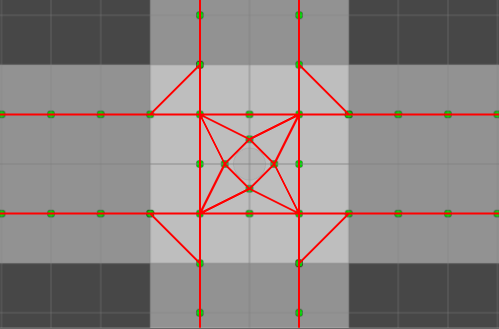
\includegraphics[scale=.4]{img/graph.png}
\caption{Image of the underlying graph representation for a four way inersection.}
\label{figure:graph}
\end{figure}

\begin{figure}
\centering
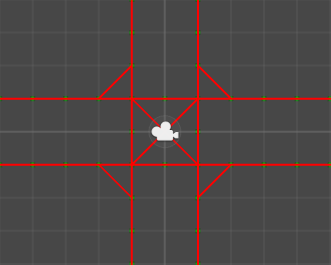
\includegraphics[height=75px]{img/graph-old1.png}
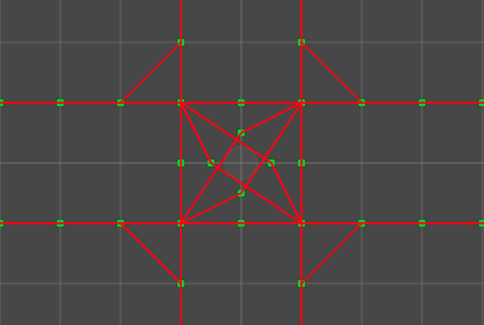
\includegraphics[height=75px]{img/graph-old2.png}
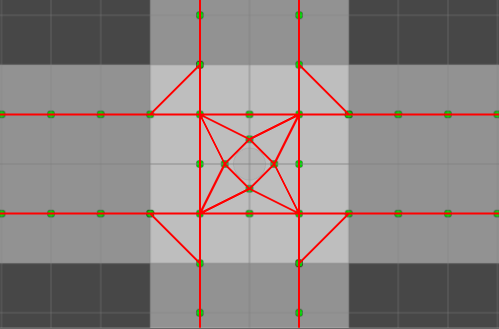
\includegraphics[height=75px]{img/graph-old3.png}
\caption{Image of the previous versions of the underlying graph representation.}
\label{figure:graphs}
\end{figure}

%We also consider a 4 way roundabout.

We represent these intersection models using an underlying directed graph.
 A car agent in our environment is seeded with information about its origin and its destination.
These points are vertices in our graph. 
Every combination of origin and destination pair has one path.

While this does not provide alot of flexibility in straying from the path, the simplicity makes the model really easy to implement and adjust.

\subsubsection{The traffic lights}
This is an attempt to mimic traffic light regulated intersections.
The lights change at intervals chosen in regards to our experiences with intersections. 
These values can vary alot from intersection to intersection - and are highly influenced by traffic flow during the day. 
We did experiments with different interval windows.

\begin{figure}
\centering
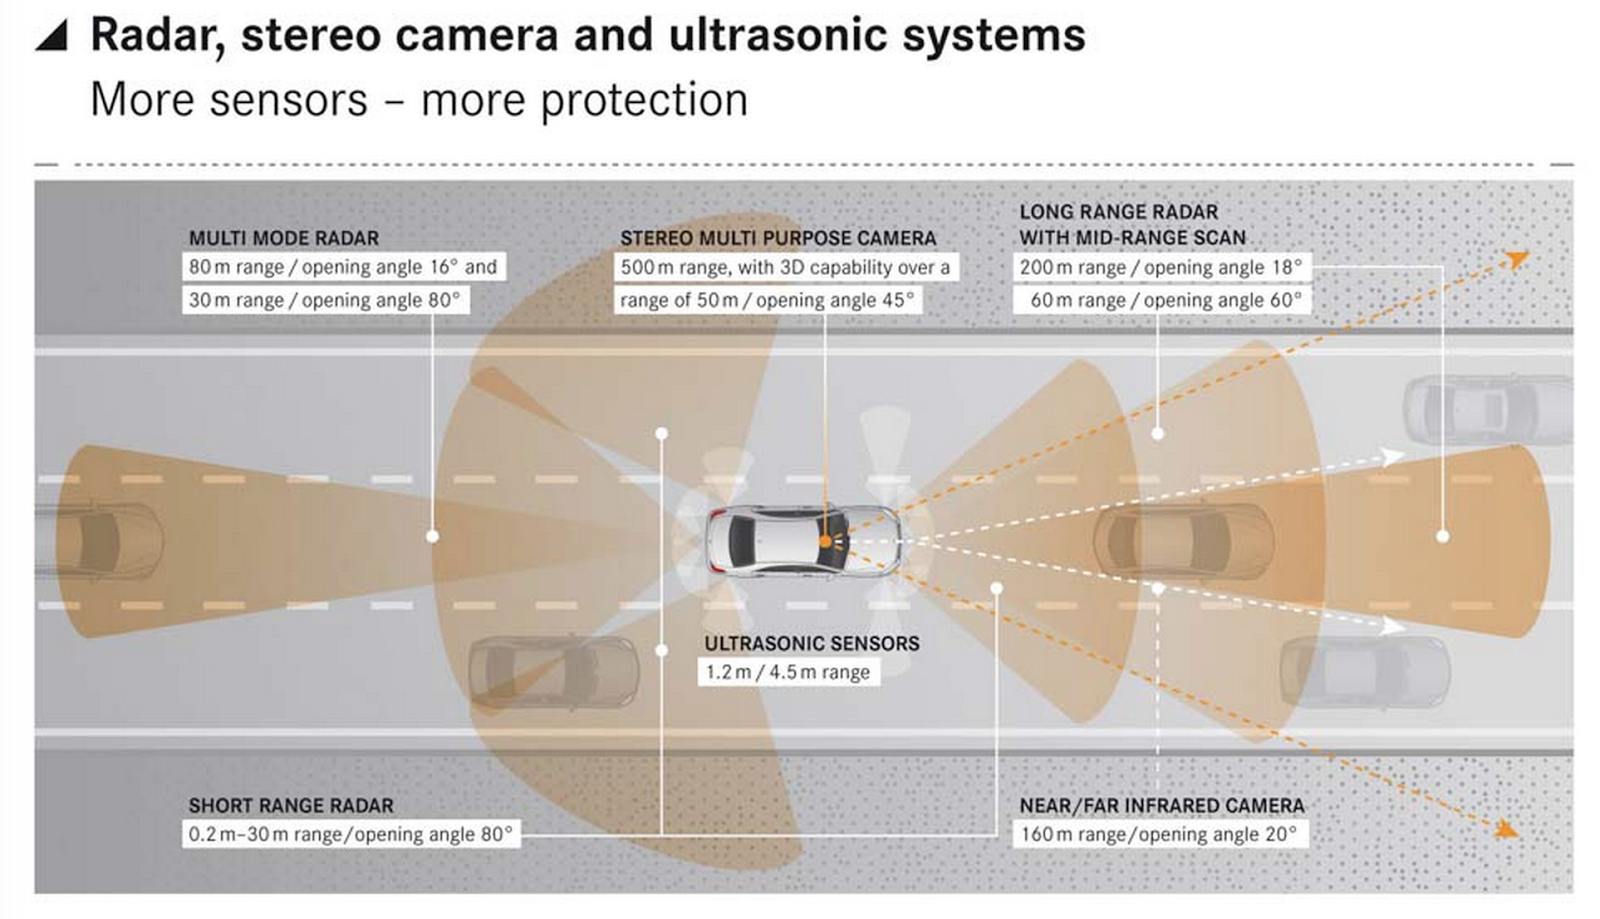
\includegraphics[scale=.2]{img/tesla_sensor}
\caption{Image of the sensors integrated into a car.}
\label{figure:tesla_sens}
\end{figure}

\subsection{The Car Model}
The way the car has been modelled is using a interface which essentially contains actions such as accellerating or decellerating, braking, and turning left or right.
This abstraction simplifies the step of going from a virtual model to a physical one.
The interface provides loose coupling between the controller and the underlying vehicle implementation.
This seperation makes it simple to develop multiple types of controllers or vehicles.

\begin{figure}
\centering
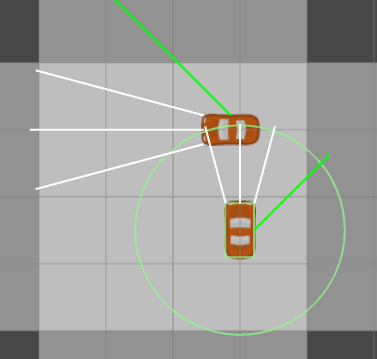
\includegraphics[scale=.5]{img/sensors}
\caption{Image of Unity sensor model.}
\label{figure:unity_sens}
\end{figure}

\subsubsection{The sensors}
Studying autonomous vehicles, such as the Tesla's we realised how much sensing is actually integrated in these marvels.
As seen on figure \ref{figure:tesla_sens}, a lot of sensors exist for achieving autonomous control in vehicles.
The figure is not representative for all autonomous vehicles - but can be seen as a good starting point for understanding the complexity of the vehicles.\\

We focused on mimicking the frontal sensors and the cross-traffic sensors.
We investigated the products of a well-known vendor, SICK, which is used by many different companies within the field.
The sensing is done similar to the current generation of autonomous vehicles. We mimick 190 degree LMS5xx series for the frontal sensor. This is a sensor which uses lasers. It provides a high degree of precision. It functions in a lot of different conditions and works in the range of 0 to 80 meters.



\subsection{The Reactive Controller}
This was developed incrementally. Initial versions were done using only collision avoidance.
The vision was to have multiple different controllers and be able to hotswap these for the simulation.
Later versions also included constructs for priority such as right hand rule. A finer grained distinction between moving objects and their movement in relation to the agent.

The controller started by initially doing collision avoidance.
This is achieved by acting directly on the frontal sensor values.
The earliest versions only had one threshold. If anything was closer than the given threshold the car would not move.
While this avoids colliding with anything infront, it does not handle obstacle avoidance very well.



We did another version which basically trails behind the car in front.
This is done using the delta distance rather than raw distance - if both vehicles move at the same speed the delta stays zero.
